\begin{block}{On the job learning}
  \begin{center}
  {\large How do you deploy a high accuracy classifier starting with zero training examples?}
  \end{center}

  \begin{center}
  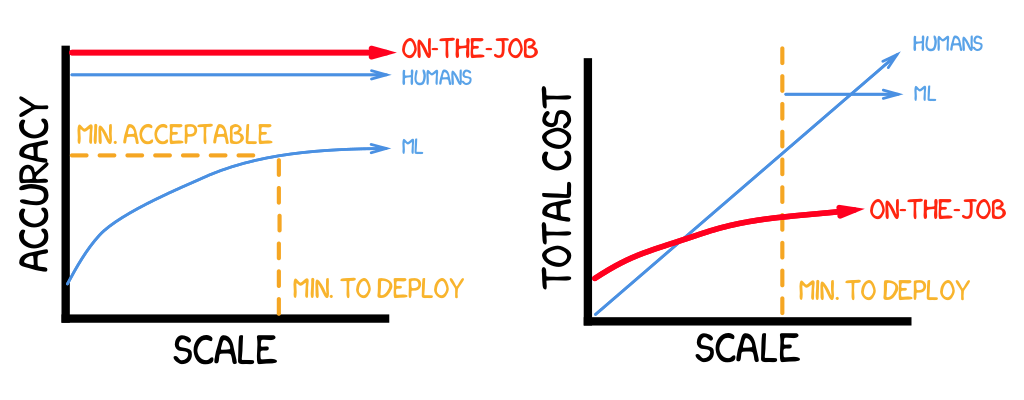
\includegraphics[width=0.8\columnwidth]{graph}
  \end{center}

  \begin{itemize}
    \item In {\bf on the job learning} when a new input arrives, the system can choose to query the crowd on \emph{parts} of the input it is uncertain about {\bf before} making a prediction. 

  \begin{center}
    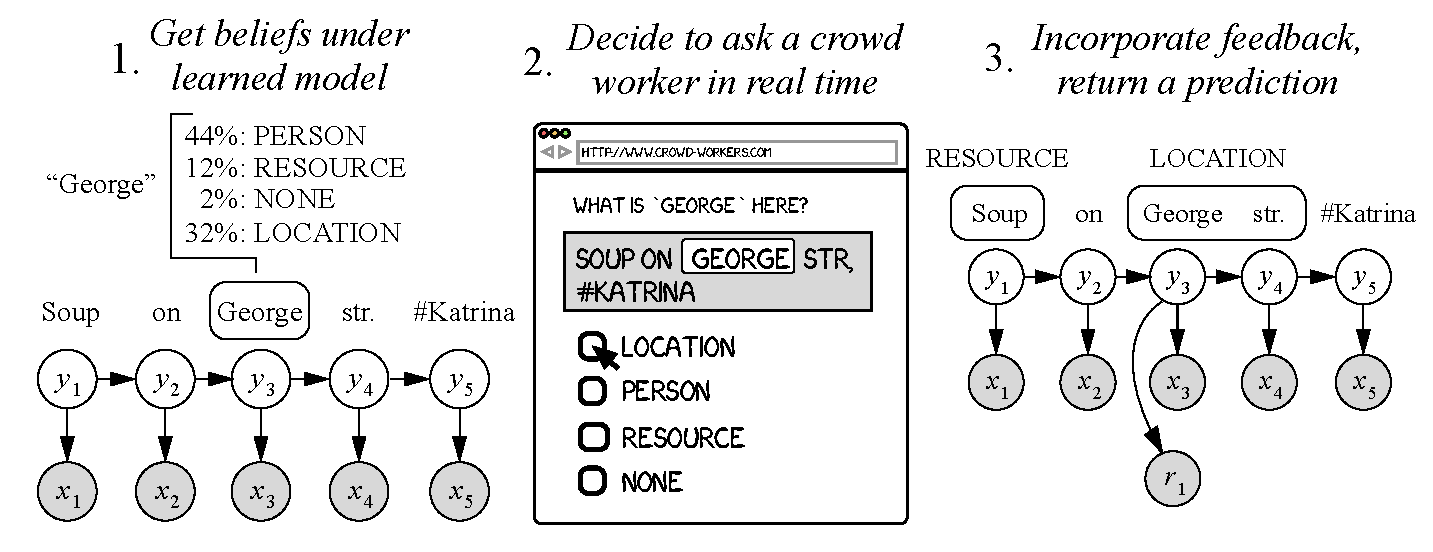
\includegraphics[width=0.8\columnwidth]{intro-banner}
  \end{center}

    \item The framework allows systems to maintain accuracy on difficult examples by asking the crowd for assistance, \emph{while} reducing costs by learning a better prediction model on-the-job.
    \item {\bf The key challenge} is how to trade off latency, cost and
      accuracy, which is modeled using {\em a game tree and Bayesian decision theory}. 
  \end{itemize}

\end{block}

\begin{block}{Related work}
  \begin{itemize}
    \item \textbf{Active learning}:
    \item \textbf{Online learning}:
  \end{itemize}
\end{block}
%\vfill

